%% LyX 2.4.4 created this file.  For more info, see https://www.lyx.org/.
%% Do not edit unless you really know what you are doing.
\documentclass[english]{article}
\usepackage[T1]{fontenc}
\usepackage[latin9]{inputenc}
\usepackage{enumitem}
\usepackage{amsmath}
\usepackage{amsthm}
\usepackage{cancel}
\usepackage{geometry}
\geometry{verbose,tmargin=1in,bmargin=1in,lmargin=1in,rmargin=1in}

\makeatletter

%%%%%%%%%%%%%%%%%%%%%%%%%%%%%% LyX specific LaTeX commands.
%% Because html converters don't know tabularnewline
\providecommand{\tabularnewline}{\\}

%%%%%%%%%%%%%%%%%%%%%%%%%%%%%% Textclass specific LaTeX commands.
\numberwithin{equation}{section}
\numberwithin{figure}{section}
\newlength{\lyxlabelwidth}      % auxiliary length 

%%%%%%%%%%%%%%%%%%%%%%%%%%%%%% User specified LaTeX commands.
\usepackage{fancyhdr}
\usepackage{lastpage}
\pagestyle{fancy}
\usepackage{enumitem}
\usepackage{ifthen}
%sets math fonts to be more readable
\everymath=\expandafter{\the\everymath\displaystyle}
%\DeclareMathSizes{10}{10}{10}{10}
\usepackage{multicol}

\usepackage{tikz}
\usetikzlibrary{plotmarks}
\usepackage{pgfplots}
\pgfplotsset{compat=newest}

\usepackage{calc}
\usepackage[nomessages]{fp}

\usepackage{advdate}    % Advancing/saving dates
\usepackage{datetime}   % Dates formatting
\usepackage{datenumber} % Counters for dates
% Added by lyx2lyx
\setlength{\parskip}{\smallskipamount}
\setlength{\parindent}{0pt}

\makeatother

\usepackage{babel}
\begin{document}
\renewcommand{\author}{Dr.\,James Ashe}

\newcommand{\classNum}{107}

\newcommand{\classSec}{7 and 10}

\newcommand{\nameType}{Name:}

\newcommand{\examType}{Quiz 1}

\renewcommand{\date}{}

%%First page's header%%%%%%%%%%%%%%%%%%%%%%
\fancypagestyle{firststyle} %%header settings for first pagr
{
	\fancyhead[L]{MTH \classNum{}(\classSec{}) \author{}\\
	\textbf{\examType{}} \date{}}
	\fancyhead[C]{\textbf{\nameType}}
	\setlength{\headsep}{14pt}
}
%%%%%%%%%%%%%%%%%%%%%%%%%%%%%%%%%%%%%%%%%%

%%Next page's header%%%%%%%%%%%%%%%%%%%%%%%
%\setlist{nolistsep}
\lhead{MTH \classNum{}(\classSec{})} 
\chead{\textbf{\nameType}} 
\cfoot{\thepage{}~of~\pageref{LastPage}} 
\setlength{\headsep}{5pt} 
%%%%%%%%%%%%%%%%%%%%%%%%%%%%%%%%%%%%%%%%%%%

%%Various settings; see the preamble for other settings%%%%%
%%\setenumerate[0]{leftmargin=12pt,itemindent=0pt,labelwidth=0pt}
\renewcommand{\labelenumi}{\textbf{\arabic{enumi}.}}
\renewcommand{\labelenumii}{\textbf{\alph{enumii}.}}
\thispagestyle{firststyle}
%%%%%%%%%%%%%%%%%%%%%%%%%%%%%%%%%%%%%%%%%%
\newcommand{\xmax}{10}
\newcommand{\xmin}{-10}
\newcommand{\xstep}{0} %must be xmin+n
\newcommand{\ymax}{10}
\newcommand{\ymin}{-10}
\newcommand{\ystep}{0} %must be ymin+n

\newcommand{\xspace}{\vspace{.75cm}}

\emph{You must show work to receive credit. Unless indicated otherwise,
each problem is worth equal value.}
\begin{enumerate}[resume]
\item Let $U=\{a,b,c,d,e,f,g,h,i,j,k\}$ be the universal set, $A=\{a,b,c,d,e,f\}$
and $B=\{a,c,e,h,j\}$. Find the indicated set.

\begin{enumerate}
\item $A\cup B$

\begin{enumerate}
\item []$=\{a,b,c,d,e,f,h,j\}$
\end{enumerate}
\item $A\cap B$

\begin{enumerate}
\item []$=\{a,c,e\}$
\end{enumerate}
\item $A'$

\begin{enumerate}
\item []$=\{g,h,i,j,k\}$
\end{enumerate}
\item $(A\cap B)'$

\begin{enumerate}
\item []$=\{b,d,f,g,h,i,j,k\}$
\end{enumerate}
\item $A\cap A'$

\begin{enumerate}
\item []$=\emptyset$
\end{enumerate}
\end{enumerate}
\end{enumerate}
\vfill
\begin{enumerate}[resume]
\item Let $A\subseteq U$ and $B\subseteq U$. If $n(U)=25$, $n(A)=10$,
$n(B)=20$, and $n(A\cap B)=5$, find the following:

\begin{enumerate}
\item $n(A')$

\begin{enumerate}
\item []$=n(U)-n(A)=15$
\end{enumerate}
\item $n(A\cup B)$

\begin{enumerate}
\item []$=n(A)+n(B)-n(A\cap B)=25$
\end{enumerate}
\end{enumerate}
\end{enumerate}
\vfill
\begin{enumerate}[resume]
\item Use the provided diagrams to shade in the region corresponding to
the indicated set.

\begin{tabular}{ccc}
\textbf{a. $A\cap B$} &  & \textbf{b. }$(A\cap B)'$\tabularnewline
%%%%A n B%%%%%
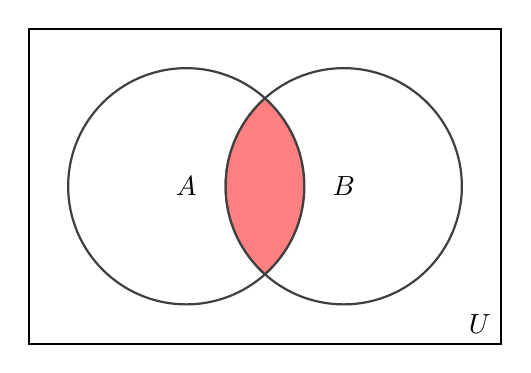
\begin{tikzpicture}[scale=1.0]
	\def\circleA{(0,0) circle (1.5)} %A
	\def\circleB{(0:2) circle (1.5)} %B

	\colorlet{circle edgeA}{black!75} 
	\colorlet{circle areaA}{red!50}
	\colorlet{circle edgeB}{black!75} 
	\colorlet{circle areaB}{red!50}

	\tikzset{
		filledA/.style={fill=circle areaA, draw=circle edgeA, thick},
		filledB/.style={fill=circle areaB, draw=circle edgeB, thick},
		outlineA/.style={draw=circle edgeA, thick},
		outlineB/.style={draw=circle edgeB, thick},
	}
	
	\begin{scope}[fill opacity=1.0]    
		\clip \circleA;     
			\fill[filledB] \circleB;
		\clip \circleB;     
			\fill[filledA] \circleA;
	\end{scope}

	\draw[outlineA] \circleA node {$A$}; 
	\draw[outlineB] \circleB node {$B$}; 
	%\node[anchor=south] at (current bounding box.north) {$A \cap B$}; 
	\draw[thick] (-2,-2) rectangle (4,2) node[anchor=south east] at (current bounding box.south east) {$U$}; 
\end{tikzpicture}  &  & \hspace{10pt}%%%%(A n B)'%%%%%
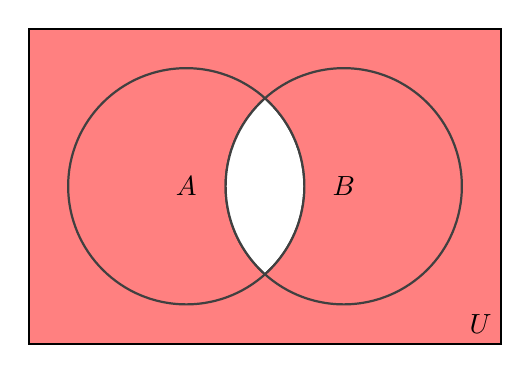
\begin{tikzpicture}[scale=1.0]
	\def\circleA{(0,0) circle (1.5)} %A
	\def\circleB{(0:2) circle (1.5)} %B

	\colorlet{circle edgeA}{black!75} 
	\colorlet{circle areaA}{white}
	\colorlet{circle edgeB}{black!75} 
	\colorlet{circle areaB}{white}

	\tikzset{
		filledA/.style={fill=circle areaA, draw=circle edgeA, thick},
		filledB/.style={fill=circle areaB, draw=circle edgeB, thick},
		outlineA/.style={draw=circle edgeA, thick},
		outlineB/.style={draw=circle edgeB, thick},
	}
	\draw[fill=red!50] (-2,-2) rectangle (4,2);

	\begin{scope}[fill opacity=1.0]    
		\clip \circleA;     
			\fill[filledB] \circleB;
		\clip \circleB;     
			\fill[filledA] \circleA;
	\end{scope}

	\draw[outlineA] \circleA node {$A$}; 
	\draw[outlineB] \circleB node {$B$}; 
	%\node[anchor=south] at (current bounding box.north) {$A \cap B$}; 
	\draw[thick] (-2,-2) rectangle (4,2) node[anchor=south east] at (current bounding box.south east) {$U$}; 
\end{tikzpicture} \tabularnewline
\textbf{c. }$A\cup B\cup C$ &  & \textbf{d. $A\cap(B\cup C)'$}\tabularnewline
\def\firstcircle{(90:1.75cm) circle (2.5cm)} 
\def\secondcircle{(210:1.75cm) circle (2.5cm)} 
\def\thirdcircle{(330:1.75cm) circle (2.5cm)}

\begin{tikzpicture}[scale=.63]    
\begin{scope}     
	\fill[red!50]\firstcircle;       
	\fill[red!50] \secondcircle;       
	\fill[red!50] \thirdcircle;     
\end{scope}     
\begin{scope}
	\clip 
	\secondcircle;       
	\fill[red!50] 
	\firstcircle;     
\end{scope}     
\begin{scope}       
	\clip 
	\secondcircle;       
	\fill[red!50] 
	\thirdcircle;     
\end{scope}     
\begin{scope}       
	\clip 
	\firstcircle;       
	\fill[red!50] 
	\thirdcircle;     
\end{scope}     
\begin{scope}       
	\clip \firstcircle;       
	\clip \secondcircle;       
	\fill[red!50] \thirdcircle;     
\end{scope}     
	\draw \firstcircle node[text=black] {$A$};    
	\draw \secondcircle node [text=black,below left] {$B$};     
	\draw \thirdcircle node [text=black,below right] {$C$};

\draw[thick] (-4.8,-3.55) rectangle (4.75,4.4) node[anchor=south east] at (current bounding box.south east) {$U$}; 

\end{tikzpicture}\hspace{10pt} &  & \def\firstcircle{(90:1.75cm) circle (2.5cm)} 
\def\secondcircle{(210:1.75cm) circle (2.5cm)} 
\def\thirdcircle{(330:1.75cm) circle (2.5cm)}

\begin{tikzpicture}[scale=.63]    
\begin{scope}     
	\fill[red!50]\firstcircle;       
	\fill[white] \secondcircle;       
	\fill[white] \thirdcircle;     
\end{scope}     
\begin{scope}
	\clip 
	\secondcircle;       
	\fill[white] 
	\firstcircle;     
\end{scope}     
\begin{scope}       
	\clip 
	\secondcircle;       
	\fill[white] 
	\thirdcircle;     
\end{scope}     
\begin{scope}       
	\clip 
	\firstcircle;       
	\fill[white] 
	\thirdcircle;     
\end{scope}     
\begin{scope}       
	\clip \firstcircle;       
	\clip \secondcircle;       
	\fill[white] \thirdcircle;     
\end{scope}     
	\draw \firstcircle node[text=black] {$A$};    
	\draw \secondcircle node [text=black,below left] {$B$};     
	\draw \thirdcircle node [text=black,below right] {$C$};

\draw[thick] (-4.8,-3.55) rectangle (4.75,4.4) node[anchor=south east] at (current bounding box.south east) {$U$}; 

\end{tikzpicture}\tabularnewline
\end{tabular}
\end{enumerate}
\vfill\newpage
\begin{enumerate}[resume]
\item A group of 100 MHU students was surveyed about the type of vehicle
they drive. 50 students like football, 40 students like basketball
and 20 students like football and basketball. Answer the following.

\begin{enumerate}
\item How many students like football or basketball?
\begin{eqnarray*}
n(F\cup B) & = & n(F)+n(B)-n(F\cap B)\\
70 & = & 50+40-20
\end{eqnarray*}
\item How many students like football but not basketball?
\begin{eqnarray*}
 &  & n(F)-n(F\cap B)\\
30 & = & 50-20
\end{eqnarray*}
\item How many students do not like football or basketball?
\begin{eqnarray*}
 &  & n(U)-n(F\cup B)\\
30 & = & 100-70
\end{eqnarray*}
\end{enumerate}
\end{enumerate}
\vfill
\begin{enumerate}[resume]
\item A group of $200$ mathematicians were asked about their pets. $70$
had dogs, $60$ had cats, $55$ had fish, $25$ owned all three, $10$
had only cats, $10$ had only dogs, and $40$ had dogs and fish. 

\begin{enumerate}
\item How many have only cats and dogs?

\begin{enumerate}
\item []$20$
\end{enumerate}
\item How many have only fish?

\begin{enumerate}
\item []$10$
\end{enumerate}
\item How many have no cats, fish,or dogs?

\begin{enumerate}
\item []$105$
\end{enumerate}
\end{enumerate}
\end{enumerate}
\begin{center}\def\firstcircle{(90:1.75cm) circle (2.5cm)} 
\def\secondcircle{(210:1.75cm) circle (2.5cm)} 
\def\thirdcircle{(330:1.75cm) circle (2.5cm)}

\begin{tikzpicture}[scale=.9]    
\begin{scope}     
	\fill[white]\firstcircle;       
	\fill[white] \secondcircle;       
	\fill[white] \thirdcircle;     
\end{scope}     
\begin{scope}
	\clip 
	\secondcircle;       
	\fill[white] 
	\firstcircle;     
\end{scope}     
\begin{scope}       
	\clip 
	\secondcircle;       
	\fill[white] 
	\thirdcircle;     
\end{scope}     
\begin{scope}       
	\clip 
	\firstcircle;       
	\fill[white] 
	\thirdcircle;     
\end{scope}     
\begin{scope}       
	\clip \firstcircle;       
	\clip \secondcircle;       
	\fill[white] \thirdcircle;     
\end{scope}     
\draw 
	\firstcircle node[text=black] {$D$} node[above=10pt] {$10$};     
\draw 
	\secondcircle node [text=black,below left] {$C$} node[below left=10pt] {$10$};     
\draw 
	\thirdcircle node [text=black,below right] {$F$} node[below right=10pt] {$10$};     
\begin{scope}[font=\small]       
	\node(0,0) {$25$}; %AnBnC       
	\draw(30:1.5cm) node {$15$}; %AnC       
	\draw(150:1.5cm) node {$20$}; %AnB       
\draw(270:1.5cm) node {$5$}; %BnC    
\end{scope}

\draw[thick] (-4.8,-3.55) rectangle (4.75,4.4) node[anchor=south east] at (current bounding box.south east) {$U$} node[anchor=north west] at (current bounding box.north west) {$105$}; 

\end{tikzpicture}

\end{center}

\vfill
\end{document}
